\chapter*{Jak Fedoru získat?}

\section*{Vyzkoušet a nainstalovat}
Fedoru je možné nainstalovat jak z~běžného optického média (CD, DVD), tak pomocí flashdisku nebo přes síť. Obrazy Fedory \emph{Workstation} ke stažení ve formátu ISO jsou k~nalezení na serveru \url{fedora.cz/jak-stahnout}. Fedora \emph{Workstation} existuje primárně ve variantě označované jako 64bitová, která je současně nabízena jako výchozí (jednoduše ta, která je v~naprosté většině případů pro uživatele tou pravou). Jedná se o~tzv. \sloppy{spustitelný live obraz, takže můžete nabootovat do funkčního systému a zjistit, o~čem stažená verze Fedory je, zda plně podporuje hardware vašeho počítače a podobně.} Zásadní je, že dosud neprobíhají žádné nevratné změny. Co máte aktuálně nainstalované na svém počítači, není jakkoliv ovlivněno. Praktické. Mimochodem zmiňme, že pro rozumný (ne minimální možný) chod Fedory \emph{Workstation} je vhodný procesor o~taktu alespoň $1\,\mathrm{GHz}$, operační paměť o~velikosti $2\,\mathrm{GiB}$ a volné místo na disku $10\,\mathrm{GiB}$ spolu s~grafickou kartou umožňující hardwarovou akceleraci.

\section*{Vytvoření instalačního média}
\begin{enumerate}

\item\emph{Fedora LiveUSB creator} -- nemáte-li notebook s~optickou mechanikou, je nezbytné stažený obraz zapsat např. pomocí utility \emph{Fedora LiveUSB creator} (existuje ve variantách jak pro \emph{MS Windows}, tak pro Linux) na flashdisk. Pozor, tato operace smaže všechna data obsažená na daném flashdisku! Pomocí \emph{Fedora LiveUSB} creatoru dokonce můžeme nejprve stáhnout i samotný instalační obraz. Software je dostupný opět z~adresy: \url{fedora.cz/jak-stahnout}.

\item\emph{Jak na ISO obraz} -- naopak zcela klasickou cestou, jak vytvořit instalační médium, je vypálení ISO obrazu na DVD. Většina soudobých operačních systémů umožňuje tuto operaci už v~rámci systému jako takového, popř. je možné nainstalovat specializovanou, volně stažitelnou aplikaci (v~Linuxu např. \emph{Brasero} a analogicky na \emph{MS Windows} lze doporučit např. \emph{ImgBurn}).

\item\emph{GNOME a Disky} -- máme-li k~dispozici linuxový operační systém (nutno dodat s~nainstalovaným prostředím GNOME), jsou tu další varianty. Při běžném procházení adresářů (aplikace \emph{Soubory}) můžeme po kliknutí pravým tlačítkem na ISO obraz vybrat položku \uv{Otevřít jinou aplikací} a posléze "Zápis obrazu disku". Dojde tím ke spuštění utility Disky, pomocí které provedeme samotný zápis na flashdisk.
\end{enumerate}

\begin{figure}[t]
\begin{center}
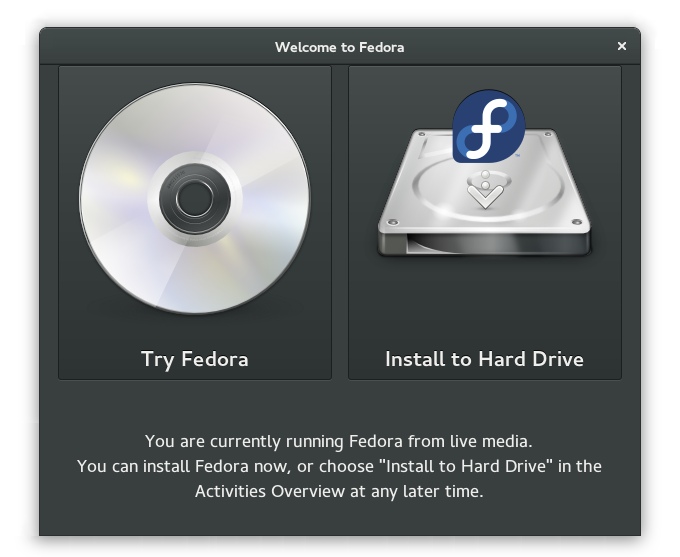
\includegraphics[width=.75\textwidth]{img/instalator-a}
\captionbelow{Nabootované instalační médium Fedory} \label{fig:instalator-a}
\end{center}
\end{figure}

Pro poslední dva body platí zásadní věc. Musíme si pečlivě ověřit, na který disk provádíme zápis instalačního ISO obrazu. Provádíme-li to na \emph{MS~Windows}, musíme ctít název diskového oddílu přiřazenému flashdisku, kam chceme zápis provést (nejčastěji \texttt{D:} či \texttt{E:}). Pod Linuxem pak musíme ověřit totéž (flashdisk bude typicky \uv{\texttt{/dev/sdX}}, kde \texttt{X} bude specifické písmeno). Asi nejlepší a nejbezpečnější cesta, jak toto zjistit, je použít aplikaci \emph{Disky}, která zobrazuje mnoho detailních informací a daném zařízení.

\section*{Instalace Fedory}
\begin{enumerate}

\item\emph{Bootování} -- \sloppy{ať už jsme si vytvořili jakékoliv bootovatelné médium, musíme se ujistit, že máme {v~BIOSu} na počítači, kde instalaci provádíme, nastavenou korektní bootovací sekvenci. Na prvním místě musí být zařízení, kde je zapsaný instalační obraz systému. Do {BIOSu} se dostaneme při spuštění počítače stiskem klávesy, která závisí na výrobci zařízení\linebreak{(typicky~\keystroke{Delete},} {\keystroke{F1},} {či~\keystroke{F2}).}} Často je také možné zvolit bootovací zařízení zcela bez vstupu do~BIOSu stiskem klávesy \keystroke{F12}.

\begin{figure}[t]
\begin{center}
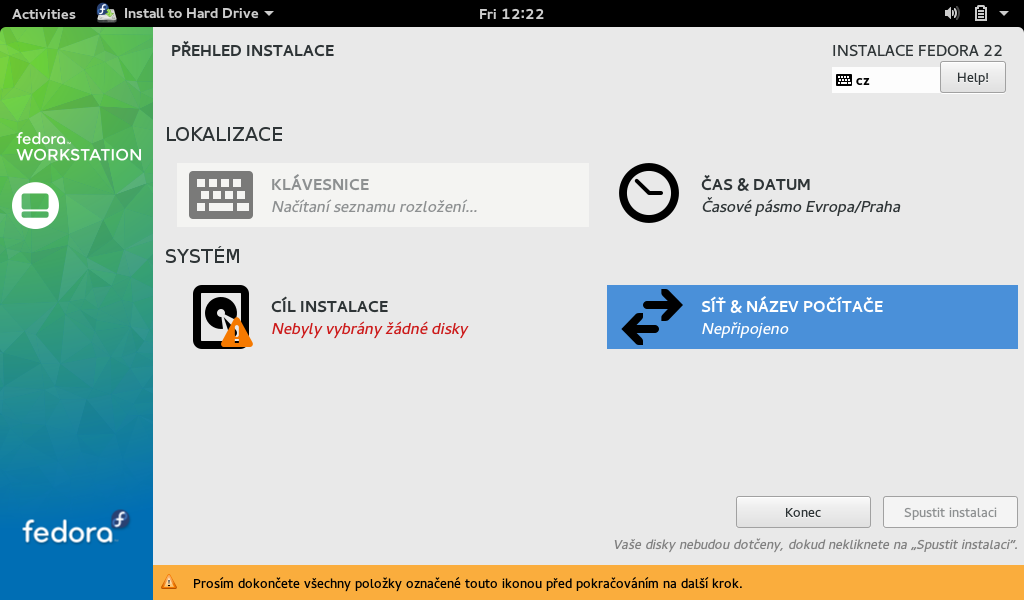
\includegraphics[width=0.95\textwidth]{img/instalator-b}
\captionbelow{Instalátor Fedory} \label{fig:instalator-b}
\end{center}
\end{figure}

\item\emph{Úvodní obrazovka} -- po úspěšném nabootování uvidíme úvodní obrazovku, kde můžeme volit primárně mezi samotnou instalaci Fedory (a bootování do živého obrazu), nebo ověřením instalačního média. Zvolíme-li instalaci, budeme zanedlouho postaveni před volbu, jestli si chceme systém vyzkoušet, nebo nainstalovat na pevný disk. První volba není fatální, Fedoru můžeme zkoušet libovolně dlouho a k~instalaci se kdykoliv vrátit přes ikonu v~menu.

\pagebreak

\item\emph{GNOME Shell} -- pokud jsme zvolili možnost vyzkoušet, uvidíme před sebou tzv. prostředí \emph{GNOME~Shell}, které je typické nahoře umístěným výrazným panelem se základními ovládacími prvky. Vlevo nahoře je klíčové tlačítko činnosti, přes které se lze dostat k~nainstalovaným aplikacím (a zmíněné možnosti instalovat systém), vpravo naopak menu relevantní zejména pro nastavení sítě a možnosti restartu či vypnutí systému.

\item\emph{Instalátor} -- když zvolíme možnost instalovat na pevný disk, jsme postupně provázeni pomocí přehledného průvodce. Volíme krok za krokem jazyková nastavení, časové pásmo, až se dostaneme k~bodu rozdělení disku. Čili k~zásadnímu bodu řešícímu, kam se Fedora fyzicky nainstaluje. Fedora nabízí automatické rozložení, při kterém oddíly vytvoří sama, a samozřejmě i rozdělení ruční. Je také možné nastavit, které oddíly budou šifrované.

\item\emph{Pevný disk} -- Fedora v~této fázi umožňuje i vytvoření tzv. dualbootu, čili provozování dvou operačních systémů v~rámci jednoho počítače. Není problém ji tak doinstalovat vedle už existující instalace \emph{MS~Windows}. V~rámci dialogu je vlevo po celou dobu k~dispozici přehled existujících oddílů. Než změny potvrdíte, pečlivě si zkontrolujte, že jsou tam všechny (např. oddíly jiných operačních systému), které tam mají být. Po odsouhlasení tohoto kroku proběhnou nevratné změny a zápis nového rozložení na disk.

\item\emph{Závěr} -- zatímco se systém instaluje, vyplníme několik zásadních údajů, jako je heslo roota (administrátora) a vytvoříme uživatelský účet, pod kterým budeme běžně pracovat (a opět mu nastavíme heslo). Pozor, Fedora uplatňuje, na rozdíl od mnoha dalších linuxových distribucí, klasický přístup k~uživatelským účtům, při kterém účet uživatele root není zakázaný. Potřebujeme tedy nastavit a znát minimálně dvě hesla. Nevyhovuje vám toto nastavení? Nevadí, i u~našeho běžného účtu můžeme zaškrtnout volbu \uv{Správce}, která nám umožní velkou část správcovské činnosti stvrdit i pod naším běžným účtem a tedy i jeho heslem.

\item\emph{A~je hotovo} -- celá instalace by neměla zabrat více než několik desítek minut. Po restartu a přihlášení provedeme ještě několik krátkých poinstalačních nastavení (a pokud jsme měnili nastavení bootování, uvedeme ho do původního stavu) a systém je připraven. Zdařilo se? Můžeme tak začít používat Fedoru v~celé její kráse!
\end{enumerate}
